\section{Smart Home Control Scenario}
To understand how our device could be used to interact with smart appliances, we also asked all study participants to work through a concrete scenario. The main goal was to obtain qualitative feedback on the usability and utility of our device with more realistic tasks.

\begin{figure}[t]
\centering
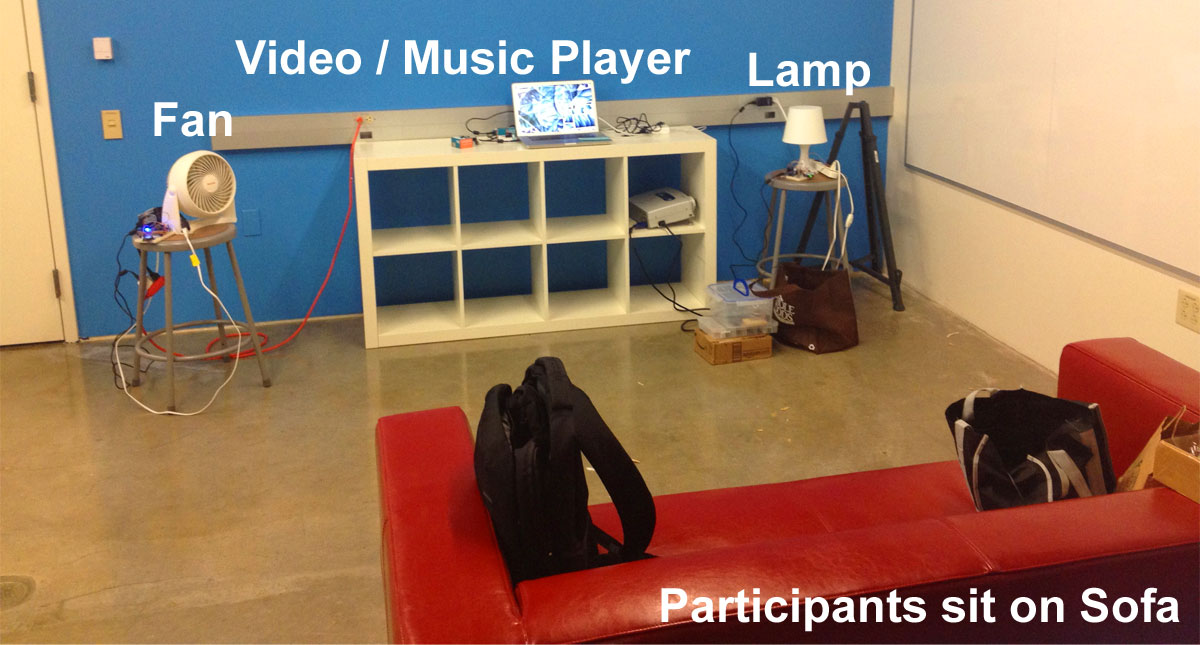
\includegraphics[width=1.0\columnwidth]{figures/smarthome-scenario.jpg}
\caption{In the smart home scenario, participants completed a series of appliance control tasks in a simulated living room.}
\label{fig:smarthome}
\end{figure}

\subsection{Methodology}
We recreated a living room environment that had three controllable appliances: a fan, a lamp, and one laptop functioning as a video player (see Figure~\ref{fig:smarthome}). The fan and lamp had binary controls: they could be switched on or off. The laptop had multiple parameterized functions: participants could start, pause, fast forward, rewind, and adjust volume.

We then asked users to work through the following script for controlling the room for watching a movie in the evening:
{\small
\begin{enumerate}
\item Turn off the lights as you want to watch the movie in a darkened room.
\item You feel a little hot in the room, so you turn on the fan.
\item You connect to the Smart TV and start playing the movie. 
\item The volume seems too soft to hear over the fan- turn it up a bit. 
\item After a while, you want to take a break to get a snack. Pause the movie. 
\item When you come back, you've forgotten what was said last - rewind by ~30 seconds and restart the movie. 
\item When the credits roll, you stop the movie and turn the lights back on.
\item After awhile, you turn off the fan and leave the room.
\end{enumerate}
}

For this study, we only elicited subjective data in the form of Likert data and open-ended responses.
\begin{figure}[b]
\centering
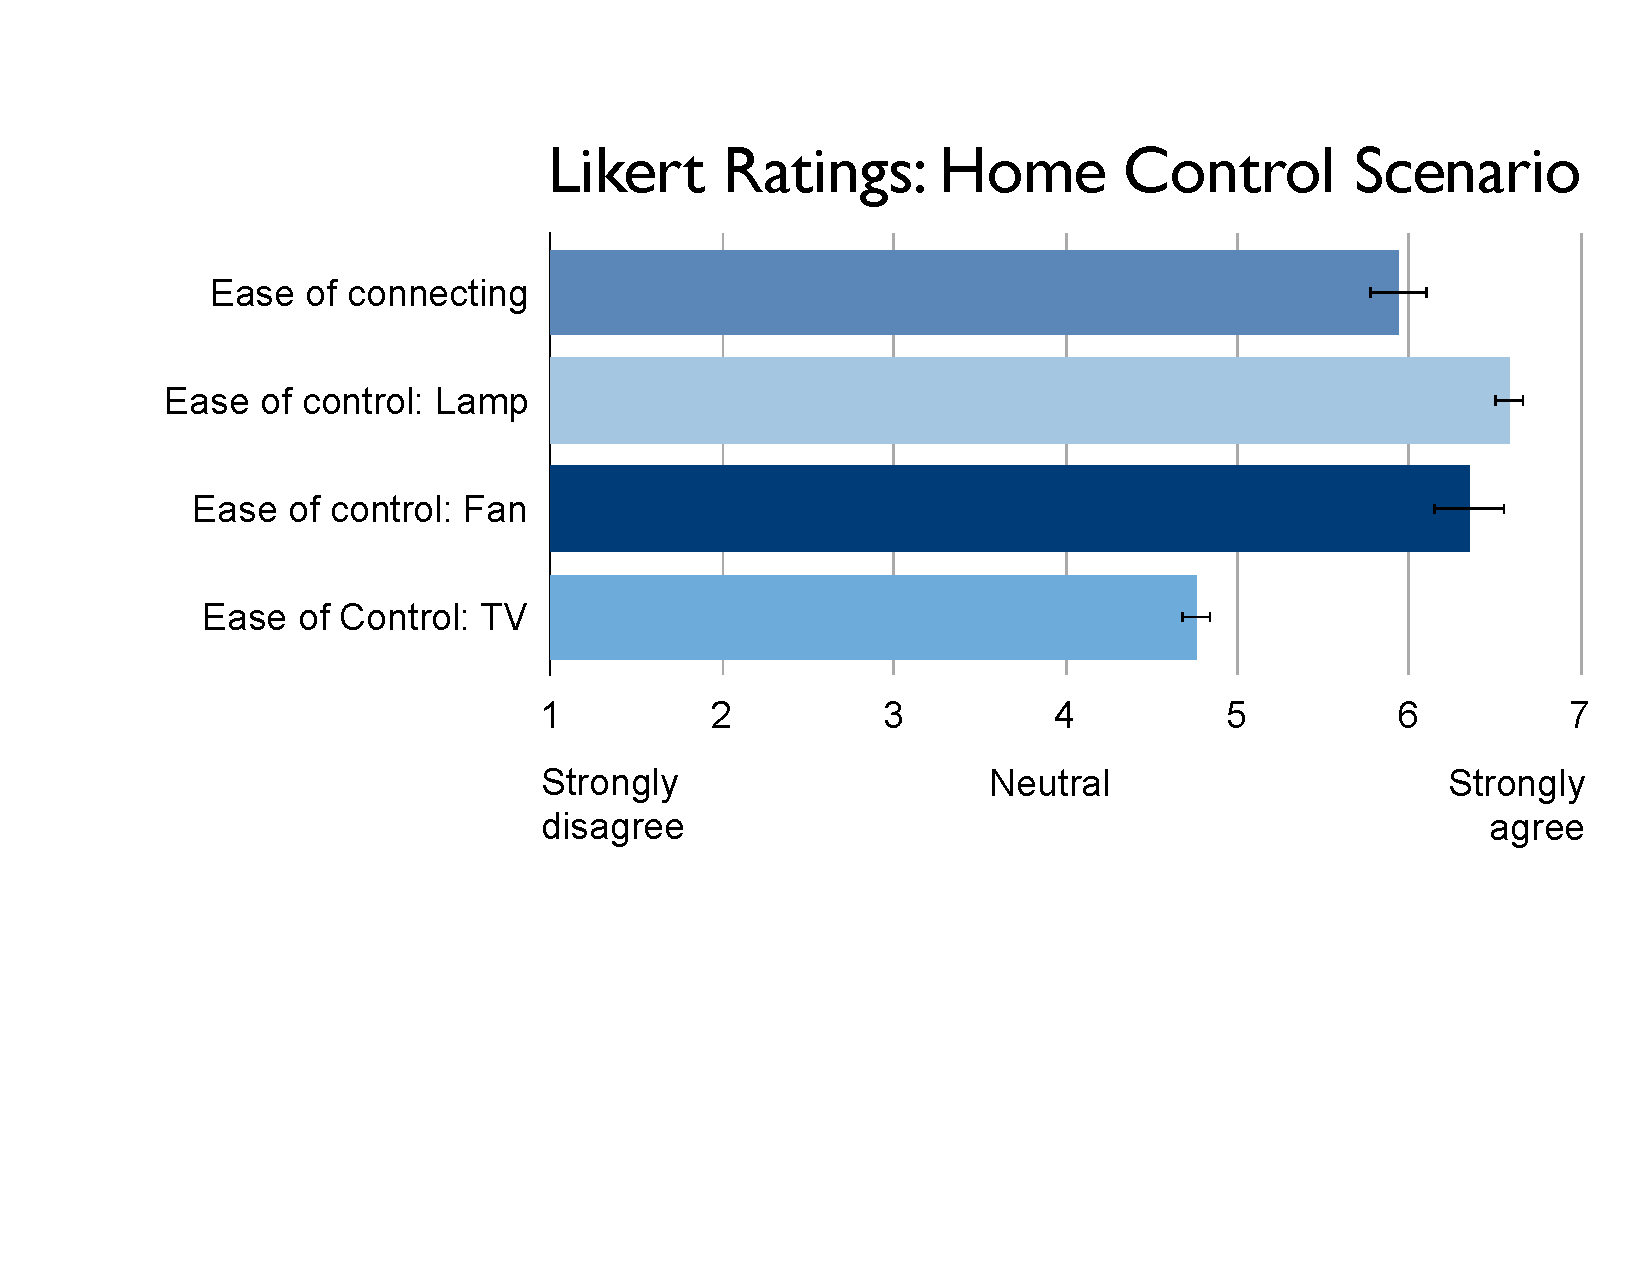
\includegraphics[width=1.0\columnwidth]{figures/scenario-likert.pdf}
\caption{Likert scale ratings for ease of use of aspects of the smart home control scenario. Error bars show standard error.}
\label{fig:smarthome-likert}
\end{figure}

\subsection{Results}
All participants successfully completed the list of tasks.
Participants stated it was easy to interact with the appliances, but there were distinct differences between appliances. Ease of use ratings were higher for the lamp and fan which had simple, discrete on/off actions, and lower for the more complex movie player (see Figure~\ref{fig:smarthome-likert}). Multiple participants remarked that the difficulty was based on the affordances of Glass: \studyquote{Most of the difficulty I had with Glass came from having to navigate the interface on the tiny screen with the touch pad}. The screen size and 1D input put a limit on the complexity of interfaces that can be presented.

\subsubsection{Visual overlap between Near-Eye Display and Target Appliance}
When a participant looks at a target, the near-eye display may occlude or overlap the target appliance. This may make it difficult to read either the on-screen display or see information displayed on the target device.  As one participant remarked \studyquote{This was especially annoying with the TV because there were two screens overlapping each other.} While it is possible to look away once a device has been acquired to better see the Glass display, this tension is likely to remain for users who want to rely on feedback from the devices themselves instead of the Glass display.



%Overall it felt easy to interact with the appliances. I imagine that moving backwards and forwards in the video by swiping could get frustrating if one were trying to move by just a little bit, or to a specific spot."
%Operating the lamp and fan felt very natural because each only involved turning it on or off, which can be done with tapping Glass once. Most of the difficulty I had with Glass came from having to navigate the interface on the tiny screen with the touch pad, but only clicking once made use a lot easier. The TV was a little more difficult to operate because there were more options on the display. Tapping felt more natural than the multi-touch gestures.
%"Again, the lack of movement is both good and bad. It's good in that you can just stay in one place and control everything.  Also, everything is centralized, so you don't need to use multiple switches. I liked the two-finger touch to change the volume as well as to fast-forward/rewind. It's clever.  The only issue with it, though, was that I felt like I didn't have as fine-grained control, but perhaps that's because I have not practiced swiping with Glass much.

%I didn't like that it promotes a sedentary lifestyle. Also, I disliked how it took away the tactile feeling that you get from pushing buttons. I didn't like how you had to scroll through a bunch of things to access certain items when otherwise I could just have flipped a switch."
%I think it's cool to control home appliances by using Glass if the home devices are far from the place where the user is. It might also be useful for people who need to take care of small children that they can complete all the tasks while keeping an eye on their children at the same time.
%it was easy to connect, but it was annoying to have to first connect to turn on/off - I kept trying to point and then immediately click to turn on/off, but I had to do the extra step of connecting THEN turning on/off.  I also tried to point back at the appliance when I was already connected.  I intuitively want the screen to automatically appear when the IR detects the appliance rather than having to tap to connect.
%"i liked the feeling i had while doing the selection etc

%i disliked that lag time where i was looking at the thing i wanted to control and it wasn't responding to me - about 500ms or so of interaction discomfort"
